\documentclass[]{article}
\usepackage[a4paper, total={7.0in, 10.5in}]{geometry}%6
\usepackage[ruled,vlined,linesnumbered]{algorithm2e}
\usepackage{listings}
\usepackage{xcolor}
\usepackage{longtable}
\usepackage{graphicx}
\usepackage{amsmath}
\usepackage{amssymb}
\usepackage{mathtools}
\usepackage{float}

\definecolor{codegreen}{rgb}{0,0.6,0}
\definecolor{codegray}{rgb}{0.5,0.5,0.5}
\definecolor{codepurple}{rgb}{0.58,0,0.82}
\definecolor{backcolour}{rgb}{0.95,0.95,0.92}

\lstdefinestyle{mystyle}{
	backgroundcolor=\color{backcolour},   
	commentstyle=\color{codegreen},
	keywordstyle=\color{magenta},
	numberstyle=\tiny\color{codegray},
	stringstyle=\color{codepurple},
	basicstyle=\ttfamily\footnotesize,
	breakatwhitespace=false,         
	breaklines=true,                 
	captionpos=b,                    
	keepspaces=true,                 
	numbers=left,                    
	numbersep=5pt,                  
	showspaces=false,                
	showstringspaces=false,
	showtabs=false,                  
	tabsize=2,
	frame=single
}

% Title Page
\title{Homework2, Algoritmi su Grafi}
\author{Enrico Cancelli, \textit{matr.} 1237293\\
	Alessandro Pegoraro, \textit{matr.} 1240466}

\begin{document}

\maketitle

\begin{abstract}

\end{abstract}

\section{Introduzione}
Lo scopo di questo  progetto è l'analisi e l'implementazione di algoritmi per la risoluzione del problema del \textit{Traveling Salesman} (in seguito TSP) su grafi completi i cui archi hanno pesi che rispettano la disuguaglianza triangolare (anche detto \textit{Triangle-TSP}).
Gli algoritmi implementati sono:
\begin{enumerate}
	\item Algoritmo (esatto) di Held e Karp
	\item Algoritmo (approssimato) di 2-approssimazione basato su MST
	\item Algoritmo (approssimato) basato su euristica costruttiva \textit{cheapest-insertion}
\end{enumerate}
\subsection{Pseudocodice}
Come riferimento per l'implementazione di questi algoritmi è stato utilizzato il seguente pseudocodice spiegato durante le lezioni di laboratorio:\\
\begin{algorithm}[H]
	\SetAlgoLined
	\DontPrintSemicolon
	\KwIn{Graph G = (V,E), S $\subseteq$ V, vertex v $\in$ S}
	\KwResult{Minimum Weight of complete path in S from 0 to v }
	\SetKwFunction{VISIT}{HK-VISIT}
	\SetKwProg{Fn}{function}{}{}
  	\Fn{\VISIT{v,S}}{
        \uIf{S = \{v\}}{
			\textbf{return} w[v,0]\;
		}
		\uElseIf{d[v,S] $\neq$ NULL}{
			\textbf{return} d[v,S]\;
		}
		\Else{
			mindist = +$\infty$\;
			minprec = NULL\;
			\For{each u $\in$ S \textbackslash \{v\}}{
				dist = HK-VISIT(u, S\textbackslash \{v\})\;
				\If{dist + w[u,v] $<$ mindist}{
					mindist = dist + w[u,v]\;
					minprec = u\;
				}
			}
			d[v,S] = mindist\;
			$\pi$[v,S] = minprec\;	
			\textbf{return} mindist\;	
		}
  	}
  	\textbf{end function}\;
	\caption{Held e Karp}
\end{algorithm}
\begin{algorithm}[H]
	\SetAlgoLined
	\DontPrintSemicolon
	\KwResult{Hamiltonial cycle}
	\SetKwFunction{VISIT}{HK-TSP}
	\SetKwProg{Fn}{function}{}{}
  	\Fn{\VISIT{G}}{
  		\textbf{let} G = (V,E)\;
  		d = Ø\;
		$\pi$ = Ø\;	
		\textbf{return} HK-VISIT(0,V)\;		
  	}
  	\textbf{end function}\;
	\caption{Initialization and call to HK-VISIT}
\end{algorithm}
\begin{algorithm}[H]
	\SetAlgoLined
	\DontPrintSemicolon
	\KwIn{Vertex v}
	\KwResult{Preorder list of MST}
	\SetKwFunction{PRE}{PREORDER}
	\SetKwProg{Fn}{function}{}{}
  	\Fn{\PRE{v}}{
  		P.add(v)\tcp*{Add v to the preorder list of MST P}
        \uIf{internal(v)}{
			\For{each u $\in$ children(v)}{
				\textbf{PREORDER}(u)\;
			}
		}
		\textbf{return} P
  	}
  	\textbf{end function}\;
	\caption{Preorder for 2-approximation}
\end{algorithm}
\begin{algorithm}[H]
	\SetAlgoLined
	\DontPrintSemicolon
	\KwIn{Graph G = (V,E), cost function c}
	\KwResult{Hamiltonial cycle}
	\SetKwFunction{APP}{APPROX\_T\_TSP}
	\SetKwProg{Fn}{function}{}{}
  	\Fn{\APP{G,c}}{
  		V = \{$v_i1$, $v_i2$, $\cdots$, $v_in$\}\;
  		r $\gets$ v1 \tcp*{Starting radix for Prim}
  		T* $\gets$ \textbf{PRIM}(G,c,r)\;
  		$<v_i1$, $v_i2$, $\cdots$, $v_in>$ = $H^\prime$ $\gets$ \textbf{PREORDER}(r)\;
		\textbf{return} $<H^\prime$, $v_in>$ = $H$\;
  	}
  	\textbf{end function}\;
	\caption{2-approximation}
\end{algorithm}
\begin{algorithm}[H]
	\SetAlgoLined
	\DontPrintSemicolon
	\KwIn{Graph G = (V,E)}
	\KwResult{Hamiltonial cycle}
	mindist = +$\infty$\; 
	j = NULL \tcp*{Find j who minimize w(0,j)}
	\For{each u $\in$ V  \textbackslash \{0\}}{
			\If{w(0,u) $<$ mindist}{
				mindist = w(0,u)\;
				j = u\;
			}
	}
	C = \{0, j, 0\}\tcp*{Repeat until the circuit has all the vertices}
	\While{$|$C $|$ $<$ $|$V $|$ + 1}{
		mindist = +$\infty$\;
		find\_i = NULL\;
		find\_j = NULL\;
		find\_k = NULL\;
		\For{each (i,j) adjacent in C}{
			\For{each k $\in$ V  \textbackslash C}{
				\If{w(i,k) + w(k,j) - w(i,j) $<$ mindist}{
					mindist = w(i,k) + w(k,j) - w(i,j)\;
					find\_i = i\;
					find\_j = j\;
					find\_k = k\;
				}		
			}
		}
	C.insertBetween(find\_i, find\_j, find\_k)\tcp*{Insert k in C between i and j}
	}
	\textbf{return} C\;
	\caption{Cheapest-Insertion}
\end{algorithm}
\section{Implementazione}
In questa sezione verranno esposte e adeguatamente motivate le scelte implementative adottate durante lo sviluppo. L'intero progetto è stato realizzato facendo il più possibile uso di codice generico (template di classe per le strutture dati di supporto e template di funzione per gli algoritmi).\\
Infine verrà data una spiegazione dettagliata sulla struttura del codice realizzato ed eventuali note per la compilazione.
\subsection{Parser}
Il dataset fornito è costituito, come per il progetto precedente, da un file per ogni grafo.\\
La struttura dei file è espressa dalla seguente formula BNF:
\begin{verbatim}
<file> :: = <name-dec>
            <type-comment block>
            <dimension>
            <edge-t-dec>
            <edge-f-dec>?
            <display-dec>?
            <coord-sec>
            EOF
<name-dec> :: = NAME: <word> \n
<type-comment block> :: = <type-dec> <comment> | 
                          <comment> <type-dec>
<type-dec> :: = TYPE: TSP \n
<comment> :: = COMMENT: <phrase> \n
<dimension> :: = DIMENSION: <integer> \n
<edge-t-dec> :: = EDGE_WEIGHT_TYPE: <edge-type> \n
<edge-type> :: = GEO | EUC_2D
<edge-f-dec> :: = EDGE_WEIGHT_FORMAT: FUNCTION \n
<display-dec> :: = DISPLAY_DATA_TYPE: COORD_DISPLAY \n
<coord-sec> :: = NODE_COORD_SECTION \n
                 <coordinates>
<coordinates> :: = <coordinate> \n
                   <coordinates> |
                   <coordinate> \n
<coordinate> :: = <integer> <float> <float>
\end{verbatim}
La classe \textit{Parser} si occupa della decodifica di questi file e organizza le informazioni rilevanti quali tipologia delle coordinate, dimensione e coordinate dei nodi creando un oggetto di classe \textit{Graph\_data}.
\subsection{Strutture dati generiche}
\subsubsection{Matrix}
La classe \textit{Matrix$<$T$>$} rappresenta una generica matrice rettangolare di oggetti di tipo T.\\
Essa è utilizzata per la memorizzazione della matrice di adiacenza associata a un grafo.
\subsubsection{MinHeap}
La struttura dati \textit{MinHeap} è la stessa utilizzata nel progetto precedente ed è utilizzata per l'esecuzione dell'algoritmo di Prim all'interno dell'algoritmo di 2-approssimazione.
\subsection{Strutture per la rappresentazione di grafi e sottoinsiemi di nodi}
\subsubsection{Graph\_Data}
Per rappresentare i dati estratti da un file relativo ad un certo grafo, abbiamo usato il template di classe \textit{Graph\_data$<$T$>$}. Gli oggetti di questo tipo contengono i seguenti campi dati:
\begin{itemize}
	\item Nome del grafo
	\item Tipo di coordinate (\verb|cartesian| o \verb|geo|)
	\item Dimensione del grafo (numero di nodi)
	\item Lista di coordinate (rappresentata come un vettore di coppie di elementi di tipo T)
\end{itemize}
Questa classe espone un unico metodo \verb|get_weights| che restituisce la matrice di adiacenza associata al grafo rappresentato dall'oggetto su cui viene invocato. La costruzione di tale matrice dipende dalla tipologia di coordinate.\\
Generalmente la matrice di adiacenza è espressa dalla seguente formula:
$$w[i,j]=dist\_fun(i, j)$$
Dove \verb|dist_fun(i,j)| è la distanza tra il nodo $i$ e $j$ del grafo.\\
In caso le coordinate di un nodo siano di tipo cartesiano, \verb|dist_fun| è la distanza euclidea:
$$dist\_fun(i,j)=round(\sqrt{((i.x - j.x)^2 + (i.y - j.y)^2)})$$
In caso le coordinate di un nodo siano coordinate geografiche, \verb|dist_fun| è la seguente funzione:
$$dist\_fun(i,j) = trunc(Earth\_Rad * acos(0.5*((1+q1)*q2-(1-q1)*q3))+1)$$
$$\text{where } q1 = cos((rad)i.y - (rad)j.y)$$
$$q2 = cos((rad)i.x - (rad)j.x)$$
$$q3 = cos((rad)i.x + (rad)j.x)$$
\subsubsection{SubSet}
\begin{flushleft}
Per tenere traccia della presenza o meno di un nodo del grafo all'interno del sottoinsieme S corrente nell'istanza dell'algoritmo \textbf{Held e Karp}, durante la ricorsione, abbiamo implementato la classe \textit{SubSet}.\\
Gli oggetti di questo tipo contengono due campi dati:
\begin{itemize}
	\item Un \verb|std::vector|$<$bool$>$ nella quale gli indici con valore \verb|TRUE| rappresentano i nodi presenti nel sottoinsieme
	\item Un contatore che traccia il numero di nodi presenti nel sottoinsieme
\end{itemize}

La classe espone i metodi \verb|at| e \verb|add| che rispettivamente permettono il controllo di presenza di un nodo nel ciclo e l'aggiunta di un nuovo nodo al ciclo.\\
Il metodo \verb|remove| è utilizzato per implementare l'operazione \verb|S\{v}| rimuovendo un nodo dal sottoinsieme e aggiornando il contatore.\\
Infine il metodo \verb|only_vertex| è utilizzato nella guardia del primo \verb|IF| dell'algoritmo di \textbf{Held e Karp}:
	\lstset{language=c++, style=mystyle,backgroundcolor=\color{white}, firstnumber=1}  	 	
\begin{lstlisting}[mathescape=true]
function HK-VISIT(v,S)
	if S = {v} then
		return w[v,0]
\end{lstlisting}
il metodo controlla se l'oggetto rappresenta un sottoinsieme singleton contenente il nodo \textit{v}.
\end{flushleft}
\subsubsection{Unordered Map}
%TODO Inserire formula di ale
%TODO ok se ho tempo la inserisco, altrimenti devi fare tu
La \verb|std::unordered_map| è l'implementazione di una \textbf{Hash Map} in \textit{C++}. Questo contenitore è stato utilizzato nell'algoritmo di \textbf{Held e Karp} per l'implementazione di \verb|d[v,S]| e $\pi$\verb|[v,S]|, dato che la complessità media di lettura e scrittura è \textit{O(1)} nel nostro caso in cui supponiamo di non avere un limite di memoria.\\
Dato che la funzione di \textbf{hashing} prende in input il nodo \verb|v| e il ciclo corrente \verb|S| rappresentato dal \verb|std::vector|$<$bool$>$ della classe \textbf{SubSet}, è risultato necessario rendere pubblico il corrispondente campo dati per ottimizzare i tempi di esecuzione.
\subsection{Algoritmi}
\subsubsection{Prim}
L'implementazione dell'algoritmo di Prim è stata realizzata nel corso dell'homework precedente. Tale algoritmo è utilizzato all'interno dell'algoritmo di 2-approssimazione ed è stato adeguatamente modificato per poter essere utilizzato con la matrice di adiacenza estratta da un oggetto \textit{Graph\_Data}.
\subsubsection{Held e Karp}
\begin{flushleft}
La nostra implementazione presente nel file \verb|algorithms\held_karp.h| è la seguente:
\lstset{language=c++, style=mystyle}
\lstinputlisting[language=c++]{held_karp.cpp}

\textbf{Note implementative:}
Come per l'algoritmo spiegato a lezione il l'implementazione si divide in due funzioni: \textbf{held$\_$karp}() che ritorna un \verb|std::vector<unsigned int>| rappresentante il circuito hamiltoniano trovato, e \textbf{held$\_$karp$\_$visit}() che calcola il circuito.\\
Per migliorare la leggibilità abbiamo definito il tipo di \textit{d}, $\pi$ e della chiave hash per la poszione \verb|[v,S]| come :
\lstset{language=c++, style=mystyle, firstnumber=1}
\begin{lstlisting}
typedef std::pair<unsigned int, std::vector<bool>> key_type;
typedef std::unordered_map<key_type, T, std::function<size_t(key_type)>> D_Map
typedef std::unordered_map<key_type, unsigned int, std::function<size_t(key_type)>> Pi_Map
\end{lstlisting}
Abbiamo anche definito il tipo del contatore per il \textbf{TIMEOUT} implementato dalla libreria \verb|std::chrono| :
\lstset{language=c++, style=mystyle, firstnumber=4}
\begin{lstlisting}
typedef std::chrono::time_point<std::chrono::steady_clock> race_time;
\end{lstlisting}
\medskip
Per l'inizializzazione di \textit{d} e $\pi$: 
\lstset{language=c++, style=mystyle,backgroundcolor=\color{white}, firstnumber=3}  	 	
\begin{lstlisting}[mathescape=true]
d = $Ø$
$\pi$ = $Ø$
\end{lstlisting}
Abbiamo ridefinito la funzione di Hashing come uno \verb|XOR| tra il vertice \verb|v| e l'hash della rappresentazione di \verb|S|
\lstset{language=c++, style=mystyle, firstnumber=35}
\begin{lstlisting}
auto hash = [](key_type a){
       return std::hash<unsigned int>()(a.first) ^ std::hash<std::vector<bool>>()(a.second);
    };
    std::unordered_map<key_type, T, std::function<size_t(key_type)>> D(1, hash);
    std::unordered_map<key_type, unsigned int, std::function<size_t(key_type)>> Pi(1, hash);
\end{lstlisting}
\medskip
Il controllo se la ricorsione ha raggiunto una foglia dell'albero o se il valore \verb|d[v,S]| è già stato calcolato :
\lstset{language=c++, style=mystyle,backgroundcolor=\color{white}, firstnumber=2}  	 	
\begin{lstlisting}[mathescape=true]
if S = {v} then
	return w[v,0]
else if d[v,S] $\neq$ NULL then
	return d[v,S]
else
\end{lstlisting}
è stato implementato in modo simile all'algoritmo spiegato a lezione utilizzando la classe \textbf{SubSet} :
\lstset{language=c++, style=mystyle, firstnumber=6}
\begin{lstlisting}
	if (S.only_vertex(v)){
        return w.at(v,0);
    }else if(D.contains(std::make_pair(v, S.collection))){
        return D.at(std::make_pair(v, S.collection));
    }else {
\end{lstlisting}
\medskip
Nella parte successiva di esplorazione dell'albero abbiamo ancora una volta cercato di avere un implementazione il più simile possibile all'algoritmo spiegato :
\lstset{language=c++, style=mystyle,backgroundcolor=\color{white}, firstnumber=6}  	 	
\begin{lstlisting}[mathescape=true]
else
	mindist = +$\infty$
	minprec = NULL
	for each u $\in$ S\{v}
		dist = HK-VISIT(u, S\{v})
		if dist + w[u,v] $<$ mindist
			mindist = dist + w[u,v]
			minprec = u
		end
	end
	d[v,S] = mindist
	$\pi$[v,S] = minprec
	return mindist
end
\end{lstlisting}
Le uniche differenze sono l'aggiunta e la rimozione di \verb|v| da \verb|S| che avvengono prima e dopo del ciclo \verb|for| :
\lstset{language=c++, style=mystyle, firstnumber=26}
\begin{lstlisting}
        S.remove(v);
        for (int u = 1; expired && ( u < w.sizeY() ); ++u) {
        	if(S.at(u)){
            	...
            }
        }
        S.add(v);
        D.insert_or_assign(std::make_pair(v, S.collection), mindist);
        Pi.insert_or_assign(std::make_pair(v, S.collection), minprec);
\end{lstlisting}
Mentre nell'algoritmo questo avviene all'interno della guardia del \verb|for| e nella chiamata ricorsiva :
\lstset{language=c++, style=mystyle,backgroundcolor=\color{white}, firstnumber=9}  	 	
\begin{lstlisting}[mathescape=true]
	for each u $\in$ S\{v}
		dist = HK-VISIT(u, S\{v})
\end{lstlisting}
Infine da $\pi$ si ricostruisce il ciclo per uniformare il tipo di ritorno tra gli algoritmi :
\lstset{language=c++, style=mystyle, firstnumber=43}
\begin{lstlisting}
    std::vector<unsigned int> C(1,0);
    SubSet Y(w.sizeY(), true);
    for(int i = 0; Pi.contains(std::make_pair(C[i], Y.collection)); ++i){
        C.push_back(Pi.at(std::make_pair(C[i], Y.collection)));
        Y.remove(C[i]);
    }
    C.push_back(0);
    return C;
\end{lstlisting}



\bigskip
\textbf{Implementazione del TIMEOUT:}
Ogni chiamata alla funzione \textbf{held$\_$karp$\_$visit}() passa con riferimento un contatore temporale \verb|starting_time| e una variabile booleana \verb|expired|.
La variabile inizialmente vale \verb|true| mentre il contatore è inizializzato alla prima chiamata della funzione all'interno di \textbf{held$\_$karp}() :
\lstset{language=c++, style=mystyle, firstnumber=40}
\begin{lstlisting}
	race_time starting_time = std::chrono::steady_clock::now();
	T value = held_karp_visit(0, S, w, D, Pi, starting_time, true);
\end{lstlisting}
\smallskip
All'interno di \textbf{held$\_$karp$\_$visit}() dopo ogni chiamata ricorsiva viene calcolato se il \textbf{TIMEOUT} (definito con \verb|#define TIMEOUT 1200.00|) è scaduto:
\lstset{language=c++, style=mystyle, firstnumber=21}
\begin{lstlisting}
	std::chrono::duration<double> now = std::chrono::steady_clock::now()-starting_time;
	if(now.count() >= TIMEOUT)
    	expired = false;
\end{lstlisting}
In caso positivo \verb|expired| viene settata a \verb|false| uscendo così dal ciclo \verb|for|.
\lstset{language=c++, style=mystyle, firstnumber=14}
\begin{lstlisting}
	for (int u = 1; expired && ( u < w.sizeY() ); ++u)
\end{lstlisting}
\medskip
Il controllo del tempo dopo la chiamata ricorsiva garantisce che anche con un \textbf{TIMEOUT} uguale a 0, almeno una foglia dell'albero sia stata raggiunta e sia stato esplorato almeno un ciclo (in questo caso dato che partiamo dal nodo 1 il ciclo è \{1, 2, ... n, 1\}).
\end{flushleft}

\newpage
\subsubsection{2-approssimazione}
\begin{flushleft}
L'algoritmo di 2-approssimazione è stato implementato nel file \verb|algorithms\preorder_2approx.h|:
\lstset{language=c++, style=mystyle}
\lstinputlisting[language=c++]{2approx.cpp}

\textbf{Note implementative:}\\
Il ciclo hamiltoniano calcolato è rappresentato come un \verb|std::vector<unsigned int>| dei vertici contenuti nel ciclo stesso.\\
L'algoritmo utilizza una funzione di supporto \verb|preorder| che, dato un MST (o in generale un albero rappresentato da una lista di adiacenza), restituisce la lista di nodi dell'albero in \textit{traversal pre-order}.
Dato un nodo di partenza \verb|f_elem|, la funzione restituisce la seguente lista definita ricorsivamente:
$$preorder(f\_elem) \triangleq [f\_elem] \dblcolon preorder(f\_elem.parent(1)) \dblcolon ... \dblcolon preorder(f\_elem.parent(n))$$
Tale definizione induttiva è implementata dal seguente frammento di codice:
\lstset{language=c++, style=mystyle, firstnumber=4}
\begin{lstlisting}
	out.emplace_back(f_elem);
	for(unsigned int i: tree[f_elem]){
		auto part = preorder(i, tree);
		out.insert(out.end(), part.begin(), part.end());
	}
\end{lstlisting}
La funzione \verb|preorder_2approx| utilizza \verb|preorder| ed implementa l'algoritmo vero e proprio.
L'algoritmo esegue questi semplici passi:
\begin{itemize}
	\item Esecuzione dell'algoritmo di Prim per ricavare il MST
	\item Esecuzione di \verb|preorder| per ricavare la lista di nodi
	\item Aggiunta del nodo 0 per chiudere il ciclo
\end{itemize}
Tali passi sono implementati nel seguente frammento di codice:
\lstset{language=c++, style=mystyle, firstnumber=13}
\begin{lstlisting}
	Tree_t mst = Prim(w);
	std::vector<unsigned int> chain = preorder(0, mst);
	chain.emplace_back(0);
\end{lstlisting}
\end{flushleft}
\newpage
\subsubsection{Euristica cheapest-insertion}
\begin{flushleft}
Come euristica abbiamo scelto \textbf{Cheapest-Insertion}, e l'implementazione presente nel file \verb|algorithms\cheapest_insertion.h| è la seguente:
\lstset{language=c++, style=mystyle}
\lstinputlisting[language=c++]{cheap_insert.cpp}

\textbf{Note implementative:}\\
La funzione come le altre ritorna un \verb|std::vector<unsigned int>| che rappresenta il circuito hamiltoniano trovato.\\
La procedura descritta a lezione è composta da 4 passi:
\begin{enumerate}
\item \textbf{Inizializzazione:} considera il circuito parziale composto dal solo vertice \verb|0|. Trova un vertice \verb|j| che minimizza \verb|w(0,j)| e costruisci il circuito parziale \verb|(0,j,0)|
\item \textbf{Selezione:} trova un vertice \verb|k| non presente nel circuito parziale e un arco \verb|{i,j}| del circuito parziale che minimizzano il valore \verb|w(i,k)+w(k,j)-w(i,j)|
\item \textbf{Inserimento:} inserisci \verb|k| tra \verb|i| e \verb|j|
\item ripeti da (\textbf{2}) finché non hai inserito tutti i vertici nel circuito
\end{enumerate}
Il passo \textbf{1} è implementato nella prima parte dell'algoritmo:
\lstset{language=c++, style=mystyle, firstnumber=2}
\begin{lstlisting}
    std::vector<unsigned int> C(2,0);
    T find_min = (T)INT_MAX;
    int find_node = -1;
    for(int j = 1; j<w.sizeY(); ++j){
        if(w.at(0,j) < find_min) {
            find_min = w.at(0, j);
            find_node = j;
        }
    }
    C.insert(C.begin() + 1, find_node);
    bool L[w.sizeY()] = {0};
    L[0], L[find_node] = true, true;
\end{lstlisting}
Prima del passo \textbf{2} inizializziamo un vettore di \verb|bool| per tenere traccia dei nodi inseriti nel ciclo parziale ad ogni iterazione:
\lstset{language=c++, style=mystyle, firstnumber=12}
\begin{lstlisting}
    bool L[w.sizeY()] = {0};
    L[0], L[find_node] = true, true;
\end{lstlisting}
Il passo \textbf{4} di ripetizione è implementato dal ciclo while:
\lstset{language=c++, style=mystyle, firstnumber=14}
\begin{lstlisting}
    while(C.size() <= w.sizeY()){
   	    ...    
    }
\end{lstlisting}
All'interno del ciclo while è implementato il passo \textbf{2}:
\lstset{language=c++, style=mystyle, firstnumber=15}
\begin{lstlisting}
        find_min = (T)INT_MAX;
        find_node = -1;
        unsigned int temp_pos = INT_MAX;
        for(int k = 1; k<w.sizeY(); ++k){
            if(!L[k]){
                for(unsigned int i = 0; i<C.size()-1; ++i) {
                    if((w.at(C[i],k) + w.at(C[i+1],k) - w.at(C[i],C[i+1])) < find_min){
                        find_min = w.at(C[i],k) + w.at(C[i+1],k) - w.at(C[i],C[i+1]);
                        find_node = k;
                        temp_pos = i+1;
                    }
                }
            }
        }
\end{lstlisting}
Cicliamo tutti i nodi del grafo che non fanno parte del circuito (saltando lo 0 dato che sappiamo faccia parte del circuito di partenza), e per ogni nodo cerchiamo quello che minimizza la formula: 
$$w(i,k)+w(k,j)-w(i,j)$$
Nel passo \textbf{3} inseriamo il nodo trovato e aggiorniamo il vettore tenente traccia dei nodi presenti nel ciclo parziale:
\lstset{language=c++, style=mystyle, firstnumber=29}
\begin{lstlisting}
        C.insert(C.begin() + temp_pos, find_node);
        L[find_node] = true;
\end{lstlisting}

\end{flushleft}
\newpage
\section{Analisi}
\subsection{Risultati prodotti}
\begin{flushleft}
Di seguito è mostrata la tabella completa dei tempi di esecuzione (ignorando il tempo utilizzato per il parsing) e degli errori relativi degli algoritmi per ogni grafo e relativo peso del ciclo hamiltoniano trovato: 

\begin{longtable}{|c|c|c|c|c|c|c|c|c|c|}
\hline
\textbf{}        & \multicolumn{3}{c|}{\textbf{Held-Karp (t\_out 20 min)}}                   & \multicolumn{3}{c|}{\textbf{Cheapest Insertion}}          & \multicolumn{3}{c|}{\textbf{2-approssimato}}              \\ \cline{2-10} 
\textbf{Istanza} & \textbf{Soluzione} & \textbf{Tempo} & \textbf{Errore} & \textbf{Soluzione} & \textbf{Tempo} & \textbf{Errore} & \textbf{Soluzione} & \textbf{Tempo} & \textbf{Errore} \\ \hline
burma14      & 3323               & 2.44453            & 0.00          & 3588               & 0.0000191          & 0.08          & 4003               & 0.0000364          & 0.20          \\ \hline
ulysses16    & 6859               & 14.6475            & 0.00          & 7368               & 0.0000253          & 0.07          & 7788               & 0.0000413          & 0.13          \\ \hline
ulysses22    & 7188               & 1202.143           & 0.02          & 7709               & 0.0000539          & 0.10          & 8308               & 0.0000877          & 0.18          \\ \hline
eil51        & 1072               & 1200.662           & 1.52          & 494                & 0.0006023          & 0.16          & 605                & 0.000194           & 0.42          \\ \hline
berlin52     & 18920              & 1200.647           & 1.51          & 9004               & 0.0006005          & 0.19          & 10402              & 0.0003238          & 0.38          \\ \hline
kroA100      & 169787             & 1200.243           & 6.97          & 24942              & 0.003957           & 0.17          & 30516              & 0.0006457          & 0.43          \\ \hline
kroD100      & 150572             & 1200.235           & 6.07          & 25204              & 0.0047127          & 0.18          & 28599              & 0.0006957          & 0.34          \\ \hline
ch150        & 49109              & 1200.121           & 6.52          & 7998               & 0.0129079          & 0.23          & 9315               & 0.0012785          & 0.43          \\ \hline
gr202        & 56533              & 1200.071           & 0.41          & 46480              & 0.032091           & 0.16          & 52615              & 0.0023568          & 0.31          \\ \hline
gr229        & 176922             & 1200.068           & 0.31          & 153896             & 0.0464426          & 0.14          & 179335             & 0.0031117          & 0.33          \\ \hline
pcb442       & 215105             & 1200.188           & 3.23          & 60834              & 0.355548           & 0.20          & 71264              & 0.0097613          & 0.40          \\ \hline
d493         & 112313             & 1200.234           & 2.21          & 39969              & 0.501974           & 0.14          & 45334              & 0.0128767          & 0.29          \\ \hline
dsj1000      & 555573000          & 1201.523           & 28.77         & 22291200           & 4.6643             & 0.20          & 25526000           & 0.048772           & 0.37          \\ \hline
\caption{\textbf{Soluzione, Tempo di esecuzione e Errore Relativo per ogni Algoritmo}}
\end{longtable}

\subsection{Analisi e conclusioni}
\subsubsection{Confronto generale su pesi dei cicli ed errori relativi}
Per paragonare gli algoritmi approssimati con l'algoritmo esatto di Held e Karp, abbiamo effettuato test imponendo un timeout di 20 minuti, in modo da rendere più preciso possibile il ciclo ricavato da quest'ultimo. Tuttavia, come si può notare dalla Figura \ref{total}, ad eccezione di qualche istanza, l'algoritmo di Held e Karp con timeout restitutisce quasi sempre l'approssimazione pessima (in certi casi con valori superiori di un ordine di grandezza rispetto a quelli restituiti dagli altri algoritmi).
\begin{figure}[H]
	\centering
	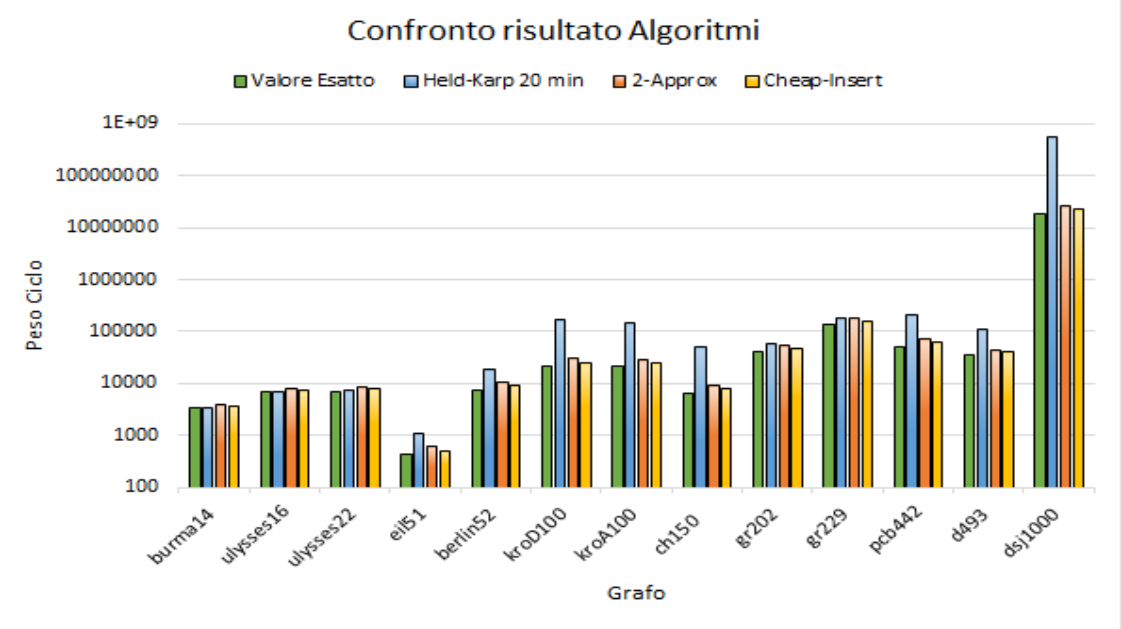
\includegraphics[width=\textwidth,height=\textheight,keepaspectratio]{CONFRONTO_RISULTATI.png}
	\caption{\textbf{Confronto degli errori relativi tra gli algoritmi}}
	\label{total}
\end{figure}
Questa differenza diventa più chiara osservando l'errore relativo delle varie soluzioni rispetto alla soluzione ottima (fornita insieme al dataset). Dalla Figura \ref{conf_tot} si può notare che, per le istanze da 14 a 22 nodi, con Held e Karp con timeout si ottiene la soluzione approssimata migliore (con errore relativo $\leq 0.02$ e per \verb|burma14| e \verb|ulysses16| la soluzione ottima).\\
Per quanto riguarda le istanze rimanenti, le soluzioni ricavate da Held e Karp superano ampiamente e quasi sempre il limite teorico di errore degli altri 2 algoritmi (essendo entrambi algoritmi di 2-approssimazione, il massimo errore relativo raggiungibile è 1).\\
Unica eccezione a questo fatto sono i risultati ottenuti per \verb|gr202| e \verb|gr229| che sono molto vicini a quelli ottenuti dall'algoritmo di 2-approssimazione.\\
Abbiamo attribuito tale evento ad una pura casualità. Essendo l'esecuzione di Held e Karp con un timeout troppo basso simile ad una visita in profondità dell'intero grafico, può accadere che tale cammino (chiuso a formare un ciclo unendo l'ultimo nodo aggiunto al nodo 1) rappresenti una soluzione approssimata abbastanza precisa.\\
\medskip
%TODO Enrico vuole completare questa parte
Confrontando invece gli algoritmi approssimati possiamo osservare come Cheapest Insertion ottenga sempre un errore relativo minore di 2-Approssimazione.
\begin{figure}[h]
	\centering
	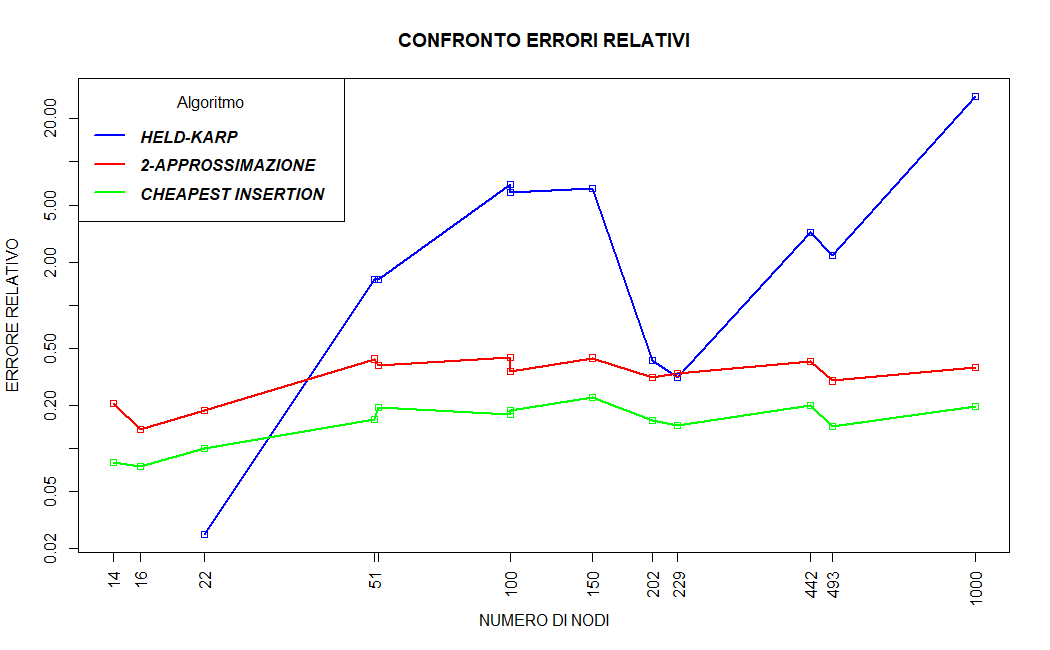
\includegraphics[width=\textwidth,height=\textheight,keepaspectratio]{CONFRONTO_ERRORI_RELATIVI_20_MIN_NEW.png}
	\caption{\textbf{Confronto degli errori relativi tra gli algoritmi}}
	\label{conf_tot}
\end{figure}
\newpage
\subsubsection{Confronto tra algoritmi di approssimazione su tempo di esecuzione}
Le due varianti di Naive Kruskal differiscono unicamente nell'approccio alla \textit{cycle detection} in fase di costruzione del MST.\\
\begin{figure}[h]
	\centering
	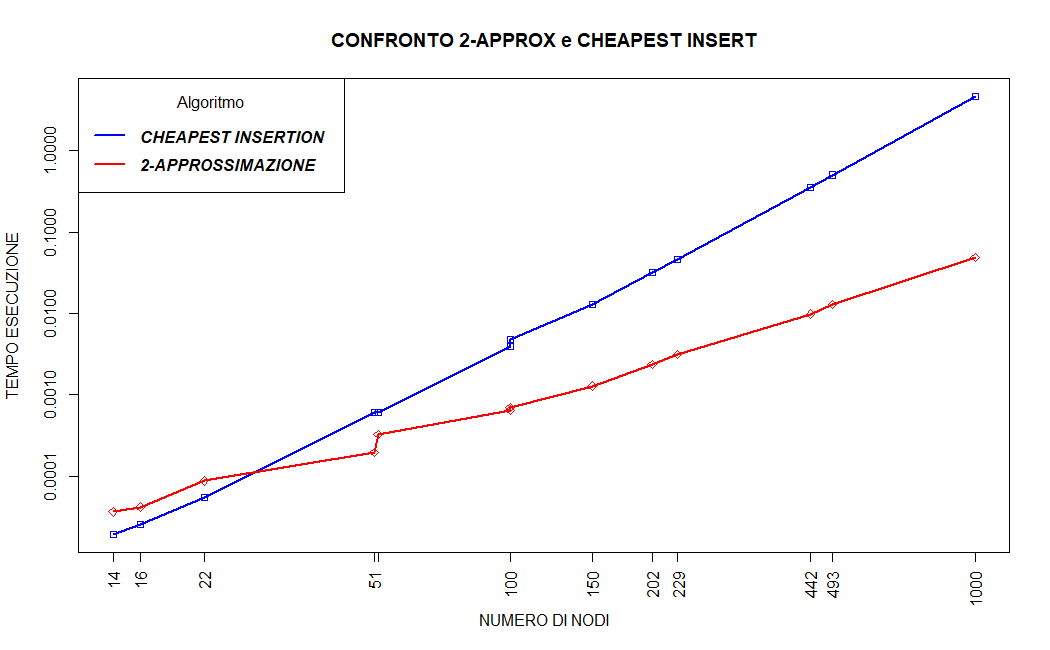
\includegraphics[width=0.9\textwidth,height=\textheight,keepaspectratio]{TEMPO_SU_NODI_2_CHEAP_NEW.png}
	\caption{\textbf{Confronto 2-Approssimazione e Cheapest Insertion}}
	\label{app-cheap}
\end{figure}

\newpage
\subsubsection{Confronto tra i TIMEOUT di Held-Karp}
Come affermato in precedenza, Kruskal Union-Find è l'algoritmo più veloce su ogni singola istanza presente nel test-set.
%TODO inserisci la tabella ale
%TODO tabella inserita
\begin{longtable}{|c|c|c|c|c|c|c|}
\hline
\textbf{TIMEOUT Held Karp} & \textbf{0 secondi} & \textbf{30 secondi} & \textbf{1 minuto} & \textbf{3 minuti} & \textbf{5 minuti} & \textbf{20 minuti} \\ \hline
Media Errore Relativo            & 4.840148           & 4.543972            & 4.513275          & 4.489914          & 4.468247          & 4.427877           \\ \hline
\caption{\textbf{Confronto variazione Errore relativo rispetto al TIMEOUT}}
\end{longtable}
\begin{figure}[h]
\centering
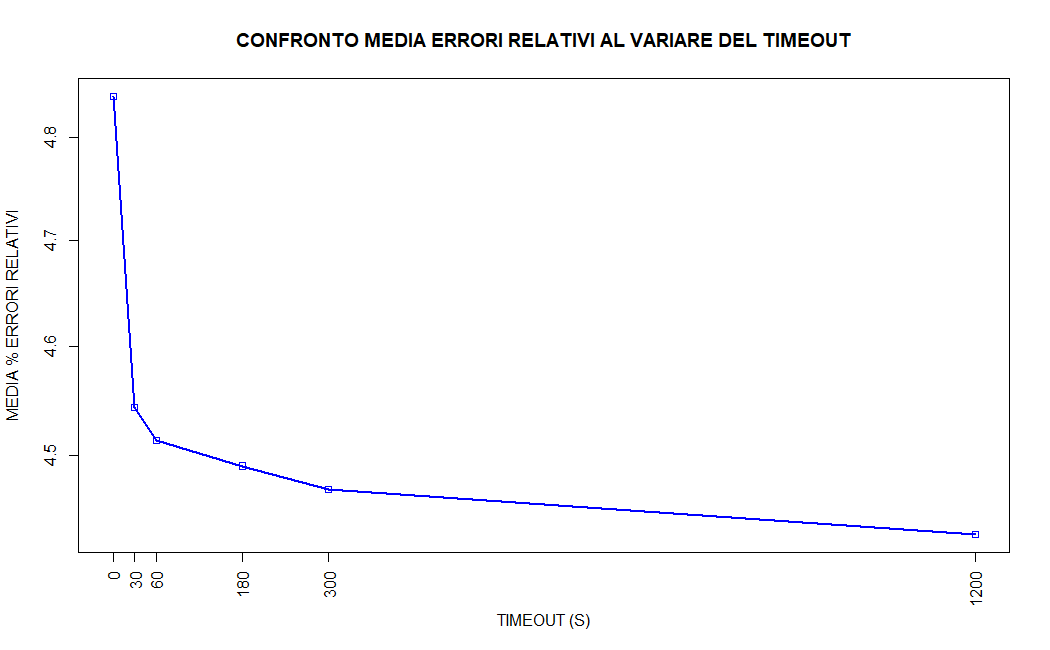
\includegraphics[width=0.9\textwidth, height=\textheight,keepaspectratio]{CONFRONTO_TIMEOUT_ERRORI.png}
\caption{\textbf{Confronto errori relativi al variare del TIMEOUT}}
\label{TIMEOUT-err}
\end{figure}

\newpage
\subsubsection{Stima dei tempi di esecuzione di Held-Karp}
%TODO trova il fattore dividendo per 2^n*n^2 e poi fai lo stesso grafico
%TODO mi sono perso cosa sia questo fattore, se ho tempo mi riguardo i grafici, altrimenti suppongo che quello da dividere per 2^n*n^2 sia il tempo stimato dato che quello si trova sull asse Y
La dimensione massima di \textit{d} e $\pi$ durante l'esecuzione dell'algoritmo di Held e Karp può essere espressa in funzione del numero di nodi $n$ del grafo:
$$max\_dim = (\sum_{k=2}^{n-1}k\cdot\binom{n-1}{k}) + 1 = 2^{(n-2)} \cdot (n-1) - (n-1) +1 = (n-1)\cdot(2^{(n-2)}-1) +1$$
Sapendo che avviene un inserimento in \textit{d} e $\pi$ ad ogni esecuzione del passo induttivo dell'algoritmo ...  supponendo di avere un computer capace di eseguire ogni chiamata ricorsiva in tempo medio $\sim 5.5*10^{-5}$ possiamo stimare il tempo di esecuzione dell'algoritmo per ogni istanza del dataset di grafi.
\begin{longtable}{|c|c|c|}
\hline
\textbf{Istanza} & \textbf{Formula tempo} & \textbf{Tempo stimato (s)}   \\ \hline
burma14.tsp      & $\sim 2.44056064$     & \textbf{2.44453}             \\ \hline
ulysses16.tsp    & $\sim 12.75068416$     & \textbf{14.6475}             \\ \hline
ulysses22.tsp    & $\sim 1542.83278336$     & \textbf{2463.33}             \\ \hline
eil51.tsp        & $(2^{51} * 51^{2}) * 7.6*10^{-7}$     & 4451267799700.45 \\ \hline				
berlin52.tsp     & $(2^{52} * 52^{2}) * 7.6*10^{-7}$     & 9255077378231.46 \\ \hline
kroA100.tsp      & $(2^{100} * 100^{2}) * 7.6*10^{-7}$     & 9634144561734543432020602642 \\ \hline
kroD100.tsp      & $(2^{100} * 100^{2}) * 7.6*10^{-7}$     & 9634144561734543432020602642 \\ \hline
ch150.tsp        & $(2^{150} * 150^{2}) * 7.6*10^{-7}$   & 2.44059355452719e+43 \\ \hline
gr202.tsp        & $(2^{202} * 202^{2}) * 7.6*10^{-7}$   & 1.99331279872149e+59 \\ \hline
gr229.tsp        & $(2^{229} * 229^{2}) * 7.6*10^{-7}$   & 3.43837756163442e+67 \\ \hline
pcb442.tsp       & $(2^{442} * 442^{2}) * 7.6*10^{-7}$   & 1.68622768133278e+132 \\ \hline
d493.tsp         & $(2^{493} * 493^{2}) * 7.6*10^{-7}$   & 4.72384123853514e+147 \\ \hline
dsj1000.tsp      & $(2^{1000} * 1000^{2}) * 7.6*10^{-7}$   & 8.14346541461563e+300 \\ \hline
\caption{\textbf{Stima del tempo di esecuzione per la soluzione esatta}}
\end{longtable}

I primi 3 tempi non sono stime ma sono stati ottenuti tramite l'esecuzione dell'algoritmo, possiamo osservare come già con 22 nodi il tempo di esecuzione si aggira intorno ai 40 minuti, ma il salto a 51 nodi porta il tempo stimato a circa 49090 anni
%TODO una conclusione??? dimostrando così l'impraticabilità dell'algoritmo per grafi di dimensioni XXX?
\begin{figure}[h]
\centering
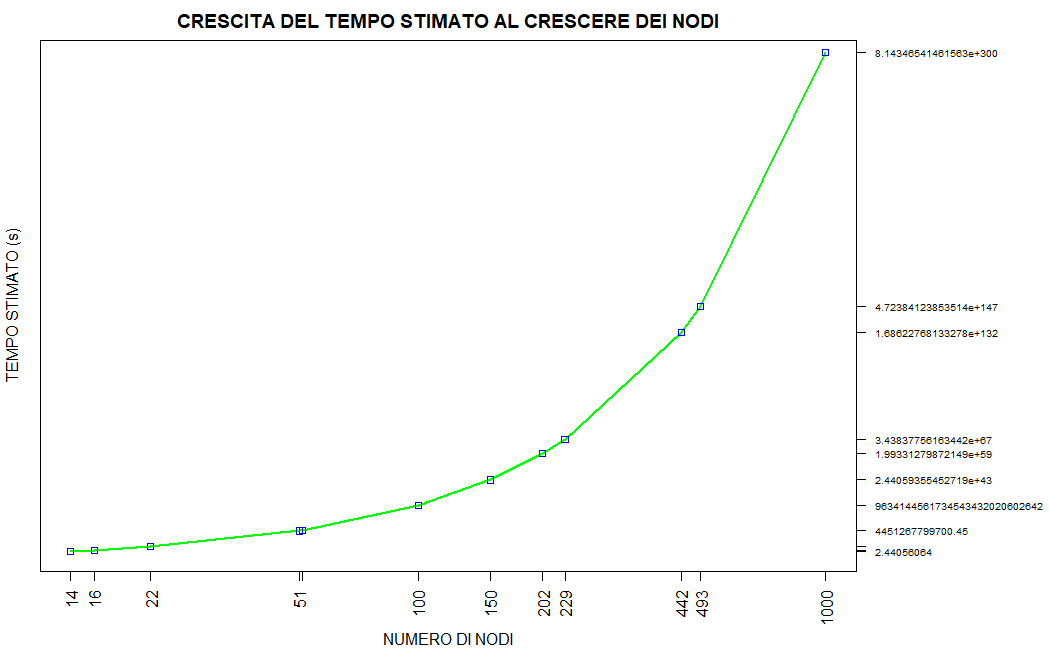
\includegraphics[width=0.9\textwidth, height=\textheight,keepaspectratio]{STIME_TEMPO.png}
\caption{\textbf{Stima della crescita del tempo di esecuzione al variare dei nodi}}
\label{STIME_temp}
\end{figure}
\end{flushleft}





\end{document}
